\subsection{Synthesis of the homocysteine thiolactone conjugates\label{sec:HCTL}}

\subsubsection{Synthesis of methyl ciprofloxacin \compound{cmpd:CipMe}}

The synthesis of the analogue conjugates began with the synthesis of methyl ciprofloxacin \compound{cmpd:CipMe} (CipMe), which would then be attached to the various head groups.
Methyl ciprofloxacin \compound{cmpd:CipMe} was synthesised from ciprofloxacin \compound{cmpd:Cip} and MeOH in good yield using \textit{para}-toluenesulfonic acid (TsOH) as a catalyst \cite{Sachin2010}.

\begin{scheme}[H]
	\begin{center}
		\schemeref[Cip]{cmpd:Cip}	
		\schemeref[CipMe]{cmpd:CipMe}
		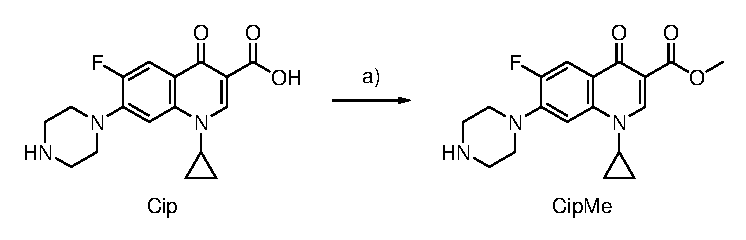
\includegraphics[scale=1]{CipMe_synth}
		\caption{Synthesis of methyl ciprofloxacin \compound{cmpd:CipMe}. a) TsOH, MeOH, 72 h, reflux, 83\%. \label{sch:CipMe_synth}}
	\end{center}
\end{scheme}

\subsubsection{Synthesis of Br-C$_4$-HCTL \compound{cmpd:SHL4Br}}

The HCTL head group was then attached to the linker to form Br-C$_4$-HCTL \compound{cmpd:SHL4Br}, in preparation for coupling to methyl ciprofloxacin \compound{cmpd:CipMe}.
Br-C$_4$-HCTL \compound{cmpd:SHL4Br} was synthesised using the Schotten-Baumann conditions employed previously for the HSL derivatives \compound{cmpd:HL4Br} and \compound{cmpd:HL6Br}. Br-C$_4$-HCTL \compound{cmpd:SHL4Br} was isolated in markedly higher yield than that achieved by Ganguly \textit{et al.}\cite{Ganguly2011} (88\% vs. 25\%). It is possible that this was due to \ce{CH2Cl2} being used for the extraction, whereas Ganguly \textit{et al.} used EtOAc.

\begin{scheme}[H]
	\begin{center}
		\schemeref[Cl4Br]{cmpd:Cl4Br}
		\schemeref[SHLHCl]{cmpd:SHLHCl}	
		\schemeref[SHL4Br]{cmpd:SHL4Br}
		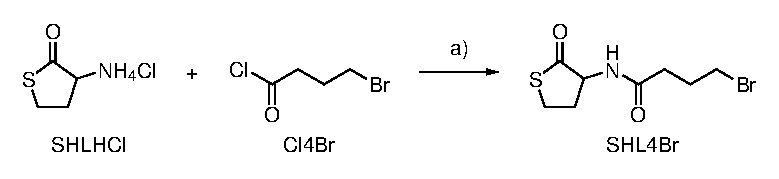
\includegraphics[scale=1]{SHL4Br_synth}
		\caption{Synthesis of Br-C$_4$-HCTL \compound{cmpd:SHL4Br}. a) \ce{NaHCO3}, \ce{CH2Cl2}, water, 0 $^{\circ}$C, 1 h, 88\%.\label{sch:SHL4Br_synth}}
	\end{center}
\end{scheme}

\subsubsection{Synthesis of the HCTL-CipMe conjugate \compound{cmpd:SHL4CipMe}}

The HCTL-CipMe conjugate \compound{cmpd:SHL4CipMe} was synthesised using the procedure outlined by Ganguly \textit{et al.}\cite{Ganguly2011} (see \ref{sch:SHL4CipMe_synth}). Monitoring by LCMS showed slow conversion to the product. Br-C$_4$-HCTL \compound{cmpd:SHL4Br} was presumably consumed by side reactions as 4 eq. were required to reach full conversion. 
A likely potential side reaction is internal cyclisation of the bromide with the amide NH, and the mass of this molecule was observed by LCMS in the reaction mixture.

Ganguly \textit{et al.} do not quote a yield for this reaction\cite{Ganguly2011,Iyer2012}, but it is hoped that the 12\% achieved here could be improved upon. The side reactions led to the production of an unidentified brown, viscous contaminant which made purification by flash column chromatography (as was used by Ganguly \textit{et al.}) challenging. Preparatory HPLC on a partially purified sample gave enough pure HCTL-CipMe conjugate \compound{cmpd:SHL4CipMe} for biological testing. Future optimisation of the synthesis could focus on different routes to the product, e.g. the peptide coupling described in \ref{sec:CipMe_linker}, or different purification methods, e.g. using just preparatory HPLC, or reverse phase flash column chromatography.



\begin{scheme}[H]
	\begin{center}
		\schemeref[CipMe]{cmpd:CipMe}
		\schemeref[SHL4CipMe]{cmpd:SHL4CipMe}
		\schemeref[SHL4Br]{cmpd:SHL4Br}
		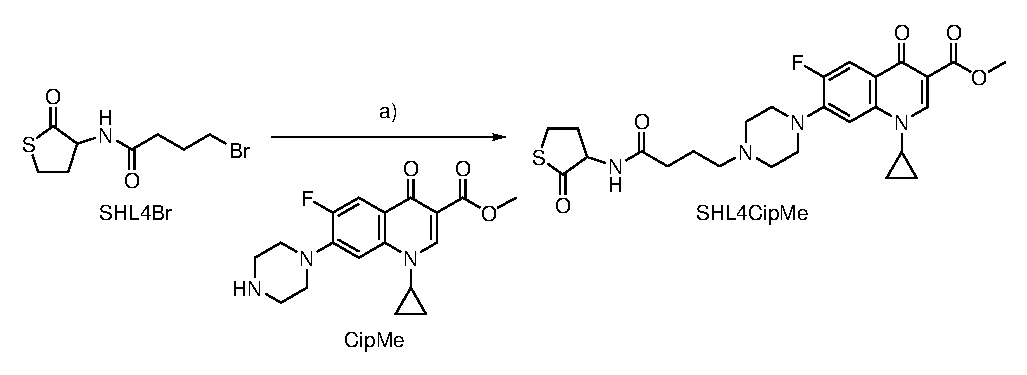
\includegraphics[scale=1]{SHL4CipMe_synth}
		\caption{
			Synthesis of the HCTL-CipMe conjugate \compound{cmpd:SHL4CipMe}.
			a) \ce{K2CO3}, acetonitrile, reflux, 24 h, 12\%.
			\label{sch:SHL4CipMe_synth}}
	\end{center}
\end{scheme}

\subsubsection{Synthesis of the HCTL-Cip triazole conjugate \compound{cmpd:SHL4T4Cip}}

Br-C$_4$-HCTL \compound{cmpd:SHL4Br} was converted into \ce{N3}-C$_4$-HCTL \compound{cmpd:SHL4N3} (see \ref{sch:SHL4CipMe_synth}), by an S$_N$2 reaction with sodium azide which proceeded in excellent yield. 

\ce{N3}-C$_4$-HCTL \compound{cmpd:SHL4N3} was then subjected to the click reaction conditions optimised previously (see \ref{sec:click_general}). The reaction proceeded very slowly at first, as the azide did not dissolve in the reaction solvent and formed a single solid clump. DMSO was added as a co-solvent, and the reaction began to proceed, albeit still slowly.  Nonetheless, the HCTL-Cip triazole conjugate \compound{cmpd:SHL4T4Cip} was isolated in good yield (see \ref{sch:SHL4T4Cip_synth}).

\begin{scheme}[H]
	\begin{center}
		\schemeref[SHL4Br]{cmpd:SHL4Br}
		\schemeref[SHL4N3]{cmpd:SHL4N3}
		\schemeref[Y4Cip]{cmpd:Y4Cip}
		\schemeref[SHL4T4Cip]{cmpd:SHL4T4Cip}
		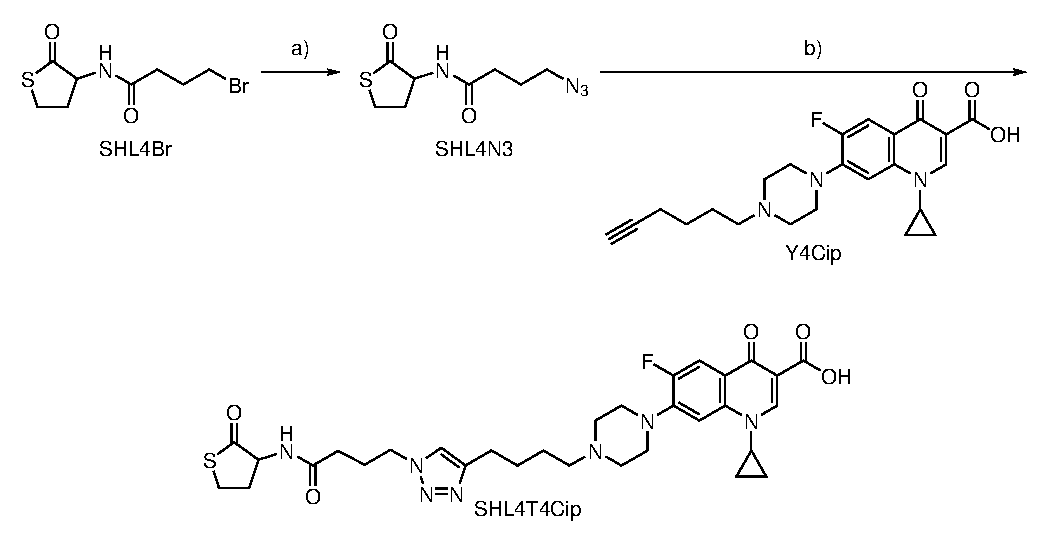
\includegraphics[scale=1]{SHL4T4Cip_synth}
		\caption{
			Synthesis of the HCTL-Cip triazole conjugate \compound{cmpd:SHL4T4Cip}.
			a) \ce{NaN3}, acetonitrile, reflux, 1.5 h, 89\%.
			b) \ce{CuSO4}, THPTA, sodium ascorbate, water, \textit{t}-BuOH, DMSO, r.t., 7 d, 71\%.
			\label{sch:SHL4T4Cip_synth}}
	\end{center}
\end{scheme}

\subsubsection{Synthesis of the cleavable HCTL-Cip triazole conjugate \compound{cmpd:SHL4THCip}}

A cleavable conjugate \compound{cmpd:SHL4THCip} (see \ref{sch:SHL4THCip_synth}) was also synthesised from \ce{N3}-C$_4$-HCTL \compound{cmpd:SHL4N3} by reaction with a cleavable alkyne-Cip derivative \compound{cmpd:Y4HCip} synthesised previously by Professor Eddy Sotelo (see \ref{sec:cleavable}).

\begin{scheme}[H]
	\begin{center}
		\schemeref[SHL4N3]{cmpd:SHL4N3}
		\schemeref[Y4HCip]{cmpd:Y4HCip}
		\schemeref[SHL4THCip]{cmpd:SHL4THCip}
		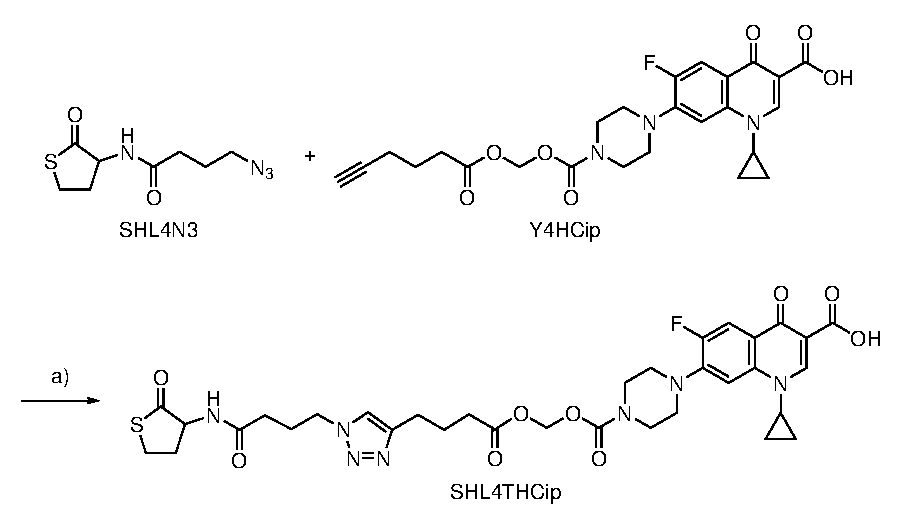
\includegraphics[scale=1]{SHL4THCip_synth}
		\caption{
			Synthesis of the cleavable HCTL-Cip triazole conjugate \compound{cmpd:SHL4THCip}.
			a) CuI, DIPEA, \ce{CH2Cl2}, r.t., 3 h, 5\%.
			\label{sch:SHL4THCip_synth}}
	\end{center}
\end{scheme}